\section{Fundamental steps of a Loop pipeline}
\label{sec:correctness-criterion}

Before, we define the three underlying fundamental steps in a loop which have the potential to distort the mappings and disturb semantic equivealence, we define a pipelinable loop and its correctness statement. 

\subsection{Definitions}
\label{sec:definitions}

\noindent
{\bf Pipelinable Loop:} Since, high level synthesis tools unroll inner loops before loop pipelining, we assume a pipelinable loop is one which has no nested loops. 
 
\smallskip
\noindent {\bf Clocked Control Data Flow Graph (CCDFG):} CCDFG is a CDFG with schedule. A CCDFG consists of basic blocks where each basic block is a sequence of steps which can be executed in a single clock cycle. Execution order within a basic block is governed by data flow. Execution order of different basic blocks is governed by control flow. The steps are represented in an assembly-level programming language. The language provides instructions for standard operations like assignment, arrays and pointer implementations etc. which are trivial to interpret. However, a construct that induces complexity is "$\phi$-statement" which we explain later in section ~\ref{sec:correctness}.

Figure~\ref{fig:pipelinable-loop}(a) represents a loop with 3 basic blocks $X$, $Y$ and $Z$. $X$ block has the exit condition $q$. If $q$ is 0, we exit the loop. Figure~\ref{fig:pipelinable-loop}(b) represents CCDFG for the loop.

\begin{figure}
\begin{center}
\begin{tabular}{c @{\hspace*{.3mm}} cc}
\begin{minipage}{.3\textwidth}
\vspace*{-2.1in}
\footnotesize
\begin{verbatim}
Entry: ...
X:
	i' = phi [i,Z] 
             [0,Entry]
	q = (i'== 3)
	i = i' + 1
	b = i + 3
	if (q == 0) GoTo Exit
	GoTo Y
Y: 
	c = a + d
Z:
	e = b + c
Exit: ...

\end{verbatim}
\normalsize

\end{minipage}
&
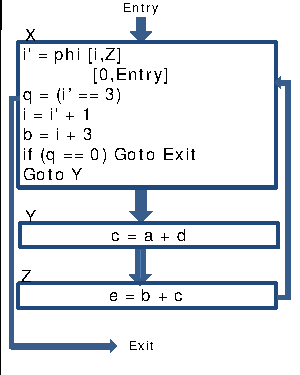
\includegraphics[height=2.2in]{fig/revised_seq_ccdfg}
\\
(a) & (b)
\end{tabular}
\end{center}
\caption{(a)Loop (b) Fragment of CCDFG corresponding to loop.  Scheduling step $X$ has a
  $\phi$-statement.}
\label{fig:pipelinable-loop}
\end{figure}

\smallskip
\noindent{{\bf Correctness Statement.}}
Let $L$ be a loop in CCDFG $C$, and let $L_{\alpha}$ be the
pipelined implementation generated by a pipeline algorithm using
pipeline parameters $\alpha$.  Let $V$ be the set of
variables in $L$, and $U$ be the set of all
variables in $C$.  Suppose we execute $L$ and $L_{\alpha}$
from CCDFG states $s$ and $s'$ respectively, such that for
each variable $v\in V$, the value of $v$ in $s$ is the same
as that in $s'$, and suppose that the state on termination
are $f$ and $f'$ respectively.  Then (1)~for any $v\in V$,
the value of $v$ in $f$ is the same as that in $f'$, and
(2)~for any $v\in(U\backslash V)$, the value of $v$ in $f'$
is the same as that in $s'$.

\medskip
\noindent
{\em Remark:} Condition (2) 
ensures that variables in $C$ that are not part of the loop
are not affected by $L_{\alpha}$.  The value of any new
variables introduced by the algorithm in $f'$ are irrelevant since they are not accessed
subsequently.

\medskip
\subsection{Correctness Criterion of Loop Pipeline}
\label{sec:correctness}

\begin{figure}
\begin{center}
\begin{tabular}{ccc}
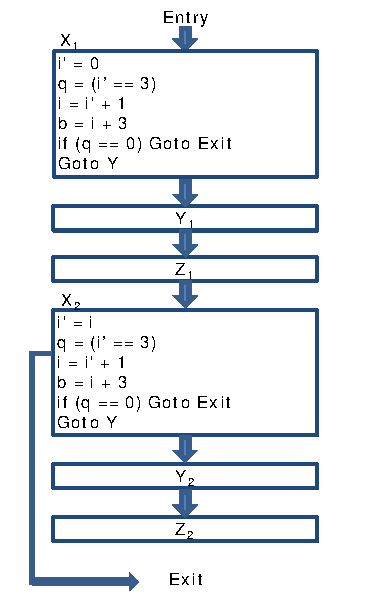
\includegraphics[height=2.2in]
{fig/phi-removal}
&
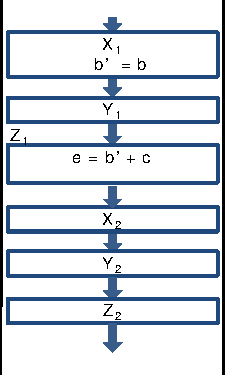
\includegraphics[height=2.2in]{fig/revised_seq_ccdfg_after_adding_shadow_registers}
&
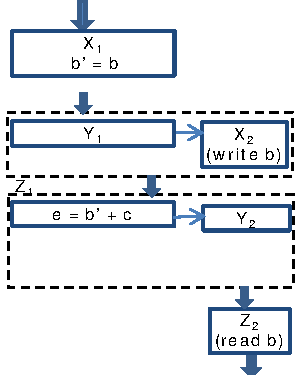
\includegraphics[height=2.2in]{fig/revised_seq_ccdfg_after_interchange}
\\
(a) & (b) & (c)
\end{tabular}
\end{center}
\caption{Components of correctness.  (a) CCDFG after unrolling the loop and replacing $\phi$ (b) after inserting
  shadow register {\tt b'} for {\tt b}. Read in
  $Z_{1}$ now occurs from {\tt b'}.  (c) Loop body
  after superstep construction.  Horizontal arrows represent
  data forwarding. Shadow register removes data-hazards, so basic blocks can be combined to create pipelined design.}
\label{fig:correctness}
\end{figure}


We claim that a correct pipelined CCDFG can be created from a sequential CCDFG through a combination of these underlying steps.

\begin{enumerate}

\item $\phi$-elimination -- A $\phi$-statement is ``{\tt v = phi
[$\sigma$ X] [$\tau$ Y]}'', where {\tt v} is a
variable, $\sigma$ and $\tau$ are expressions, and {\tt X}
and {\tt Y} are basic blocks: if it is reached from {\tt X} then it is the same as the assignment statement {\tt v = $\sigma$}; if reached from {\tt Y}, it is the same as {\tt v = $\tau$}; the meaning is undefined otherwise.
Reasoning about $\phi$-statement is complex since after its
execution from state $s$, the state reached depends not only
on $s$ but previous basic blocks in the execution history.
However, we must handle it since it is used extensively in
loops to perform different actions depending on whether the
loop body is executed the first time. One of the key pipelining steps in loop pipelining is
$\phi$-elimination i.e, unrolling the loop and replacing
$\phi$-statement with appropriate assignment statements. In figure~\ref{fig:correctness}(a), the two iterations of the unrolled loop, assign different values to variable $i'$.
	
\noindent \item \emph {shadow register step} -- A shadow register step is basically an assignment 
statement with symbol expression (x) assigned to a new value (x'). Intutively, it is correct that in a sequence of steps, if we assign a variable to a new variable and replace all occurences of x with x' till the next write of x, we should 
not have made any difference in the execution. Also, since we are not changing the value of x itself, the state after end of execution for both ccdfgs as far as real variables are conncerned (all variables excluding all shadow variables ) is same. In figure~\ref{fig:correctness}(b), if we assign a shadow register $b'$ value of $b$ at the end of $X_1$ block and replace the read occurence of b in $Z_1$ by writing the step $ e = c + b' $, the sequential execution remains same.
But, because of this step now, the two iterations have virtually independent variables, $b$ and $b'$. 

\item \emph{Superstep construction} -- This operation entails combining the scheduling steps of the successive iterations, forming scheduling ``supersteps'' that act as scheduling steps for the pipelined implementation.  The result for our example is shown in
Figure~\ref{fig:correctness}(c).  Supersteps must
account for read-after-write hazards, i.e, if a variable is written in a scheduling step $X$ and read subsequently in
$Z$ then $Z$ cannot be in a superstep that precedes $X$ in the control/data flow.  Note that we implement data forwarding (forward value of data within a single clock cycle); thus $X$ and $Z$ can be in a single superstep.

\end{enumerate}
	
\medskip
\subsection{An ongoing proof of the correctness criterion}
\label{sec:proof}	
Our correctness statement naturally breaks into correctness of $\phi$-elimination, shadow register insertion, and superstep construction.
The $\phi$-elimination theorem reduces to showing that our
algorithm correctly replaces $\phi$-statements with
assignments.  Note that this is not trivial since the algorithm has to use static analysis to
deduce the previous basic block.  Correctness of shadow
registers requires verifying similar static
analysis (\eg, to determine the subsequent read of a
variable after each write. For superstep construction, we need to verify that we can interchange any two adjacent steps which do not have any data dependencies or read-write conflict by static analysis. A series of interchanges can result in a whole block being moved up to create pipeline. 

We aim to formally verify each of these separately. Then we propose to prove the pipelining algorithm using a combination of these steps.

